% ==============================================================================
% Chapter 5: Cheat sheet - all no-brain formulas
% ==============================================================================
\section{Cheat Sheet (Read This Before the Exam)}

\subsection{Powers of two}

\begin{center}
\begin{tabular}{|c|c|c|c|c|c|c|c|}
\hline
$2^4$ & $2^5$ & $2^6$ & $2^7$ & $2^8$ & $2^9$ & $2^{10}$ & $2^{16}$ \\
\hline
16 & 32 & 64 & 128 & 256 & 512 & 1024 & 65536 \\
\hline
\end{tabular}
\end{center}

\subsection{Value ranges}

\begin{center}
\begin{tabular}{|c|c|c|}
\hline
Bits & Unsigned & Signed \\
\hline
8 & 0$\sim$255 & $-128\sim+127$ \\
10 & 0$\sim$1023 & $-512\sim+511$ \\
16 & 0$\sim$65535 & $-32768\sim+32767$ \\
\hline
\end{tabular}
\end{center}

\subsection{Fast arithmetic notes}

\begin{center}
\fbox{\parbox{0.9\linewidth}{
\textbf{Unsigned overflow:} result \% $2^N$

\textbf{Signed overflow:} if result $> 2^{N-1}-1$, subtract $2^N$

\textbf{Two's complement for negative:} $2^N - |X|$

\textbf{Two's complement to value:} MSB=1? value $-2^N$
}}
\end{center}

\subsection{K-Map positions}

\begin{center}
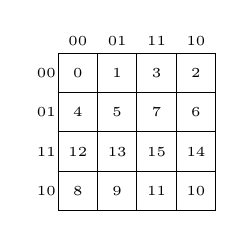
\begin{tikzpicture}[scale=0.5]
\draw (0,0) grid (4,4);
\node at (0.5, 4.3) {\tiny 00};
\node at (1.5, 4.3) {\tiny 01};
\node at (2.5, 4.3) {\tiny 11};
\node at (3.5, 4.3) {\tiny 10};
\node at (-0.3, 3.5) {\tiny 00};
\node at (-0.3, 2.5) {\tiny 01};
\node at (-0.3, 1.5) {\tiny 11};
\node at (-0.3, 0.5) {\tiny 10};
\node at (0.5,3.5) {\tiny 0};
\node at (1.5,3.5) {\tiny 1};
\node at (2.5,3.5) {\tiny 3};
\node at (3.5,3.5) {\tiny 2};
\node at (0.5,2.5) {\tiny 4};
\node at (1.5,2.5) {\tiny 5};
\node at (2.5,2.5) {\tiny 7};
\node at (3.5,2.5) {\tiny 6};
\node at (0.5,1.5) {\tiny 12};
\node at (1.5,1.5) {\tiny 13};
\node at (2.5,1.5) {\tiny 15};
\node at (3.5,1.5) {\tiny 14};
\node at (0.5,0.5) {\tiny 8};
\node at (1.5,0.5) {\tiny 9};
\node at (2.5,0.5) {\tiny 11};
\node at (3.5,0.5) {\tiny 10};
\end{tikzpicture}
\end{center}

\textbf{Order:} 00-01-11-10

\textbf{Group sizes:} 1,2,4,8,16

\textbf{Corners can be grouped!}

\subsection{RS latch}

\begin{center}
\begin{tabular}{|cc|c|}
\hline
S & R & Q \\
\hline
0 & 0 & Hold \\
0 & 1 & 0 \\
1 & 0 & 1 \\
1 & 1 & Forbidden \\
\hline
\end{tabular}
\end{center}

\textbf{Mnemonic:} S high $\Rightarrow$ Q high, R high $\Rightarrow$ Q low

\subsection{Shannon expansion}

\begin{center}
\fbox{$F = \bar{A}F_0 + AF_1$}
\end{center}

$F_0$: set $A=0$, set $\bar{A}=1$

$F_1$: set $A=1$, set $\bar{A}=0$

\subsection{Pipeline matching}

\begin{center}
\begin{tabular}{|l|l|}
\hline
Data Hazard & Forwarding \\
Load-Use & Stall \\
Branch & Flush \\
\hline
\end{tabular}
\end{center}

\textbf{CPI} = 1 + stall rate

\textbf{5-stage:} IF-ID-EX-MEM-WB

\subsection{Boolean algebra}

\begin{center}
\begin{tabular}{|l|l|}
\hline
$\overline{A+B}=\bar{A}\bar{B}$ & De Morgan \\
$\overline{AB}=\bar{A}+\bar{B}$ & De Morgan \\
$A+AB=A$ & Absorption \\
$A+\bar{A}B=A+B$ & Complement trick \\
$A\oplus B=A\bar{B}+\bar{A}B$ & XOR \\
\hline
\end{tabular}
\end{center}

\vfill
\begin{center}
\textbf{\large Good Luck!}

\small 2026-01-13 10:00 | KN-A-310

\textit{Stay calm. You've got this.}
\end{center}
